% !TEX TS-program = pdflatex
% !TEX encoding = UTF-8 Unicode

% This is a simple template for a LaTeX document using the "article" class.
% See "book", "report", "letter" for other types of document.

\documentclass[11pt]{article} % use larger type; default would be 10pt

\usepackage{polski}
\usepackage[utf8]{inputenc} % set input encoding (not needed with XeLaTeX)

\usepackage{graphicx}
%%% Examples of Article customizations
% These packages are optional, depending whether you want the features they provide.
% See the LaTeX Companion or other references for full information.

%%% PAGE DIMENSIONS
\usepackage{geometry} % to change the page dimensions
\geometry{a4paper} % or letterpaper (US) or a5paper or....
% \geometry{margin=2in} % for example, change the margins to 2 inches all round
% \geometry{landscape} % set up the page for landscape
%   read geometry.pdf for detailed page layout information

\usepackage{graphicx} % support the \includegraphics command and options

% \usepackage[parfill]{parskip} % Activate to begin paragraphs with an empty line rather than an indent

%%% PACKAGES
\usepackage{booktabs} % for much better looking tables
\usepackage{array} % for better arrays (eg matrices) in maths
\usepackage{paralist} % very flexible & customisable lists (eg. enumerate/itemize, etc.)
\usepackage{verbatim} % adds environment for commenting out blocks of text & for better verbatim
\usepackage{subfig} % make it possible to include more than one captioned figure/table in a single float
% These packages are all incorporated in the memoir class to one degree or another...

%%% HEADERS & FOOTERS
\usepackage{fancyhdr} % This should be set AFTER setting up the page geometry
\pagestyle{fancy} % options: empty , plain , fancy
\renewcommand{\headrulewidth}{0pt} % customise the layout...
\lhead{}\chead{}\rhead{}
\lfoot{}\cfoot{\thepage}\rfoot{}

%%% SECTION TITLE APPEARANCE
\usepackage{sectsty}
%\allsectionsfont{\sffamily\mdseries\upshape} % (See the fntguide.pdf for font help)
% (This matches ConTeXt defaults)

%%% ToC (table of contents) APPEARANCE
\usepackage[nottoc,notlof,notlot]{tocbibind} % Put the bibliography in the ToC
\usepackage[titles,subfigure]{tocloft} % Alter the style of the Table of Contents
\renewcommand{\cftsecfont}{\rmfamily\mdseries\upshape}
\renewcommand{\cftsecpagefont}{\rmfamily\mdseries\upshape} % No bold!

\usepackage{caption}
\usepackage{capt-of}
\usepackage{float}
%\usepackage[capposition=top]{floatrow}
%%% END Article customizations

%%% The "real" document content comes below...

\title{Waloryzacja przyrodnicza gminy wiejskiej Zgierz metodą bonitacji punktowej}
\author{Marcin Małagowski}
%\date{} % Activate to display a given date or no date (if empty),
         % otherwise the current date is printed 

\begin{document}
\maketitle

\section{Wprowadzenie}

W pracy przedstawiam analizę atrakcyjności przyrodniczej gminy wiejskiej Zgierz. Wybór obszaru badań podyktowany był wysokim zróżnicowaniem pokrycia terenu -- obecność skrzyżowań dróg krajowych, zabudowy podmiejskiej, kompleksów wypoczynkowych, terenów rolniczych oraz w pełni zalesionych.

\section{Opis metody}

Metoda bonitacji punktowej jest popularną metodą klasyfikacji i oceny obszarów. Polega ona na przydzielaniu punktów na podstawie wcześniej zdefiniowanych kryteriów. Na badany obszar powinna zostać nałożona siatka dzieląca teren na równe pola podstawowe, które podlegają ocenie.

\section{Kryteria oceny}

Ze względu na wysoką wiarygodność bazy pokrycia terenu Corine, posłużyła ona jako źródło danych do niniejszej pracy. Klasy poziomu drugiego bazy Corine są dostatecznie szczegółowe i adektwatne do potrzeb analizy obszaru wielkości gminy bądź powiatu. W tabeli \ref{tab1} zostały ujęte wybrane kryteria.

\begin{center}
\captionof{table}{Zestawienie przyjętych kryteriów}
\label{tab1}
\begin{tabular}{|r|r|r|}
\hline
Poziom 2 Corine & Punkty & Kody Corine\\
\hline
zabudowa miejska & -20 & 111-112 \\  
tereny przemysłowe i komunikacyjne & -30 & 121-124 \\
grunty orne & 15 & 211-213 \\
łąki i pastwiska & 20 & 231 \\
lasy & 25 & 311-313 \\ 
wody śródlądowe & 15 & 511-512 \\
\hline
\end{tabular}
\end{center}

\begin{figure}[H]
\centering
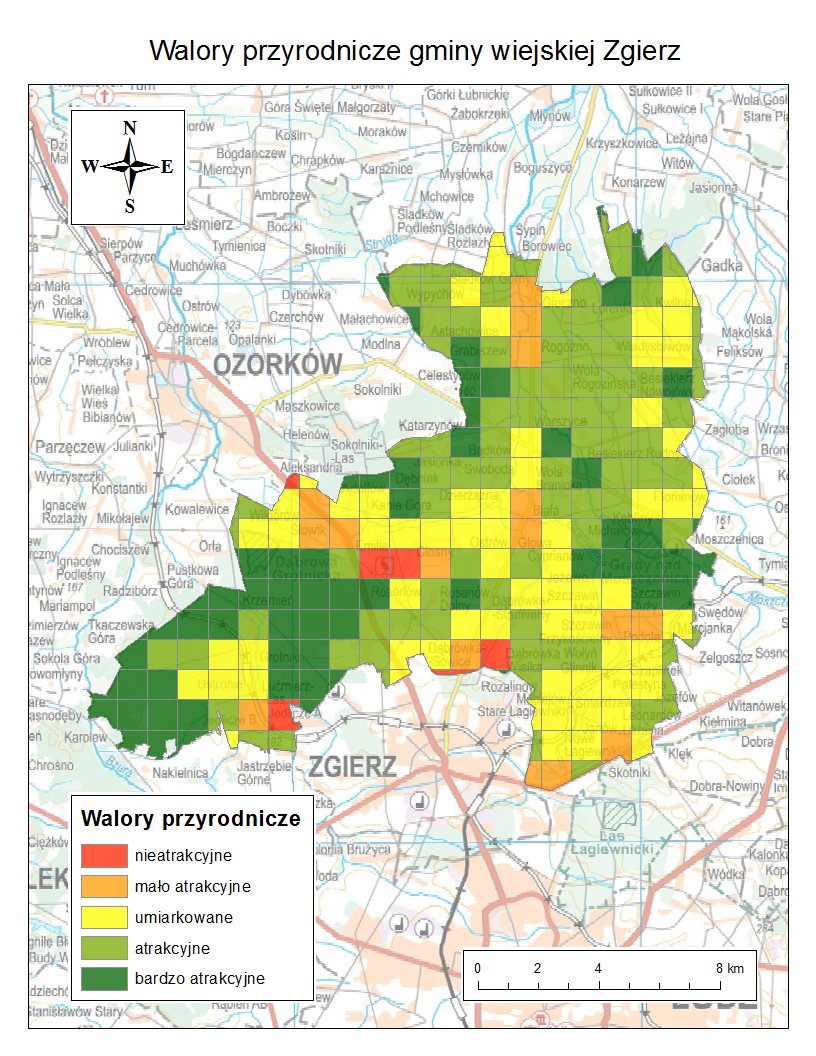
\includegraphics[scale=0.65]{final-ptbon.png}
\end{figure}

\section{Analiza wyników}

Na uwagę zasługuje bardzo wysoka ocena płd-wsch obszaru gminy obejmującego grotnicki kompleks leśny. Na jego terenie znajdują się również obszary policzone jako umiarkowanie atrakcyjne, głównie ze względu na sklasyfikowanie w Corine jako ``miejskie tereny zielone i wypoczynkowe``. Ten poziom Corine nie był jednym z kryteriów analizy stąd, pomimo rzeczywistej atrakcyjności terenu, nie otrzymał bonusu punktowego.

Wysoko atrakcyjne wydają się również okolice Swędowa na zachodzie gminy, Rosanowa w centrum oraz Kaniej Góry na północy dzięki wysokiemu zalesienu. Północ gminy z kolei charakteryzuje się dużą ilościa gruntów ornych i pastwisk co przekłada się na dość wysokie walory przyrodnicze.

Najniższe oceny otrzymał teren w bezpośrednim sąsiedztwie Zgierza z uwagi na gęstą zabudowę podmiejską. Równie niskie noty uzyskały obszary przylegające do drogi krajowej nr 91 cechujące się też przydrożną zabudową.


\end{document}
